\section{Introduction}

For a quantum computer, multiple qubits are needed that are capable of interacting with each other. 
Thus, we need to make an array of the tweezers described in \cref{ch:tweezer}, spaced from each other in the order of micrometers. 
This can be done by sending several laser beams to the objective, each under slightly different angles. 
Experimentally, this could be realized using an \ac{AOD}: a device that diffracts light off of a sound wave in a crystal, where the degree of diffraction is controlled by a \ac{RF} signal. 
By using 2 AODs in an orthogonal configuration, each supplied by a superposition of RF signals (see \cref{fig:CrossAOD}), 2D arrays of optical tweezer were successfully realized \cite{Manuel2016}. 

Nevertheless, one drawback of this method is that there is little flexibility in varying the individual laser spot intensities because of the crossed configuration.
Therefore, it was proposed to use holography methods for producing arrays of optical tweezers instead \cite{Bergamini2004}, making use of a \acf{SLM}.
Using an SLM for tweezer arrays has the advantage that it is possible to dynamically adapt the hologram, correcting for variation within trap depths of the array \cite{Nogrette2014}. 
At the same time, SLMs also allow for the correction of optical aberrations introduced by the optics in the setup \cite{Bijnen2015}.
Lastly, using the holographic method, it is even possible to make 3D arrays of tweezers \cite{DiLeonardo2007,Barredo2016}, though we will limit ourselves to 2D arrays in this work.

In the following section \ref{sec:SLM} we will introduce the working principle of the SLM, as well as the algorithm used to compute the holograms needed.
Next, in \cref{sec:SLMoperatoin} we elaborate how we used the SLM in the practice. 
Finally, in \cref{sec:ArraysResults} we present the measured spot arrays.



\section{The Spatial Light Modulator}\label{sec:SLM}

A spatial light modulator is in essence a device that can imprint a computer generated hologram onto a beam of light, allowing the spatial shaping of this light.
Different types of SLMs can manipulate properties of light like amplitude, phase and polarization.
In this work a phase-only reflective SLM was used, which as the name suggests can only control the local phase of the incoming light field.
The use of phase-only SLMs has been extensively covered in our group by, for example by \cite{Bijnen2015,Dijk2012,Bijnen2013}. 

The modulating works by deploying a pixel array, where each pixel houses a liquid birifringent crystal.
By applying a voltage (electric field) over the pixel, the orientation of the liquid crystal molecules change, changing their effective refractive index.
This principle is sketched in \cref{fig:LCoS}.
Because the crystals are birifringent they posses refractive indices along perpendicular axes, commonly referred to as the ordinary and extraordinary refractive indices respectively ($n_o$ and $n_e$). 
If the light travels a distance $t$ in a crystal unit of the SLM, the phase retardation will be $\phi_o = k t n_o$ and $\phi_e(V) = k t n_e(V)$ respectively (only the extraordinary axis can be modulated), such that the phase retarder can be represented by the Jones matrix \cite{Guzman2017}

\begin{equation}\label{eq:JonesMatrix}
    \mathbf{M} = e^{i \phi_0} 
    \begin{pmatrix}
        e^{i(\phi_e-\phi_o)} & 0\\
        0 & 1
    \end{pmatrix}.
\end{equation}
After multiplying \cref{eq:JonesMatrix} with an input electric field with components along the ordinary and extraordinary axes $\mathbf{E}_{\text{in}} = (E_e, E_o)$, it becomes clear only the component along the extraordinary axis picks up a phase retardation $\phi$ which is as a function of the voltage \cite{Guzman2017}

\begin{equation}\label{eq:ElectroOpticResponse}
    \phi(V) = \phi_e(V) - \phi_o =  k t[n_e(V) - n_0]  = \frac{2\pi}{\lambdaup}t \Delta n(V).
\end{equation}
In \cref{eq:ElectroOpticResponse} we used the birefringence parameter $\Delta n$.
The ordinary polarization axis does not pick up phase modulation, which is why typically the incident field is aligned with the extraordinary axis.
To obtain voltage control over each individual pixel, the display is manufactured on a layer of silicon, making use of various semiconductor manufacturing technologies.
As a result of diffraction from the various pixels, one can create arbitrary intensity patterns in the focal plane of a lens.
This concept is sketched in \cref{fig:SLMLens} and further explained in the next section.


\begin{figure}
	\begin{subfigure}{.39\textwidth}
		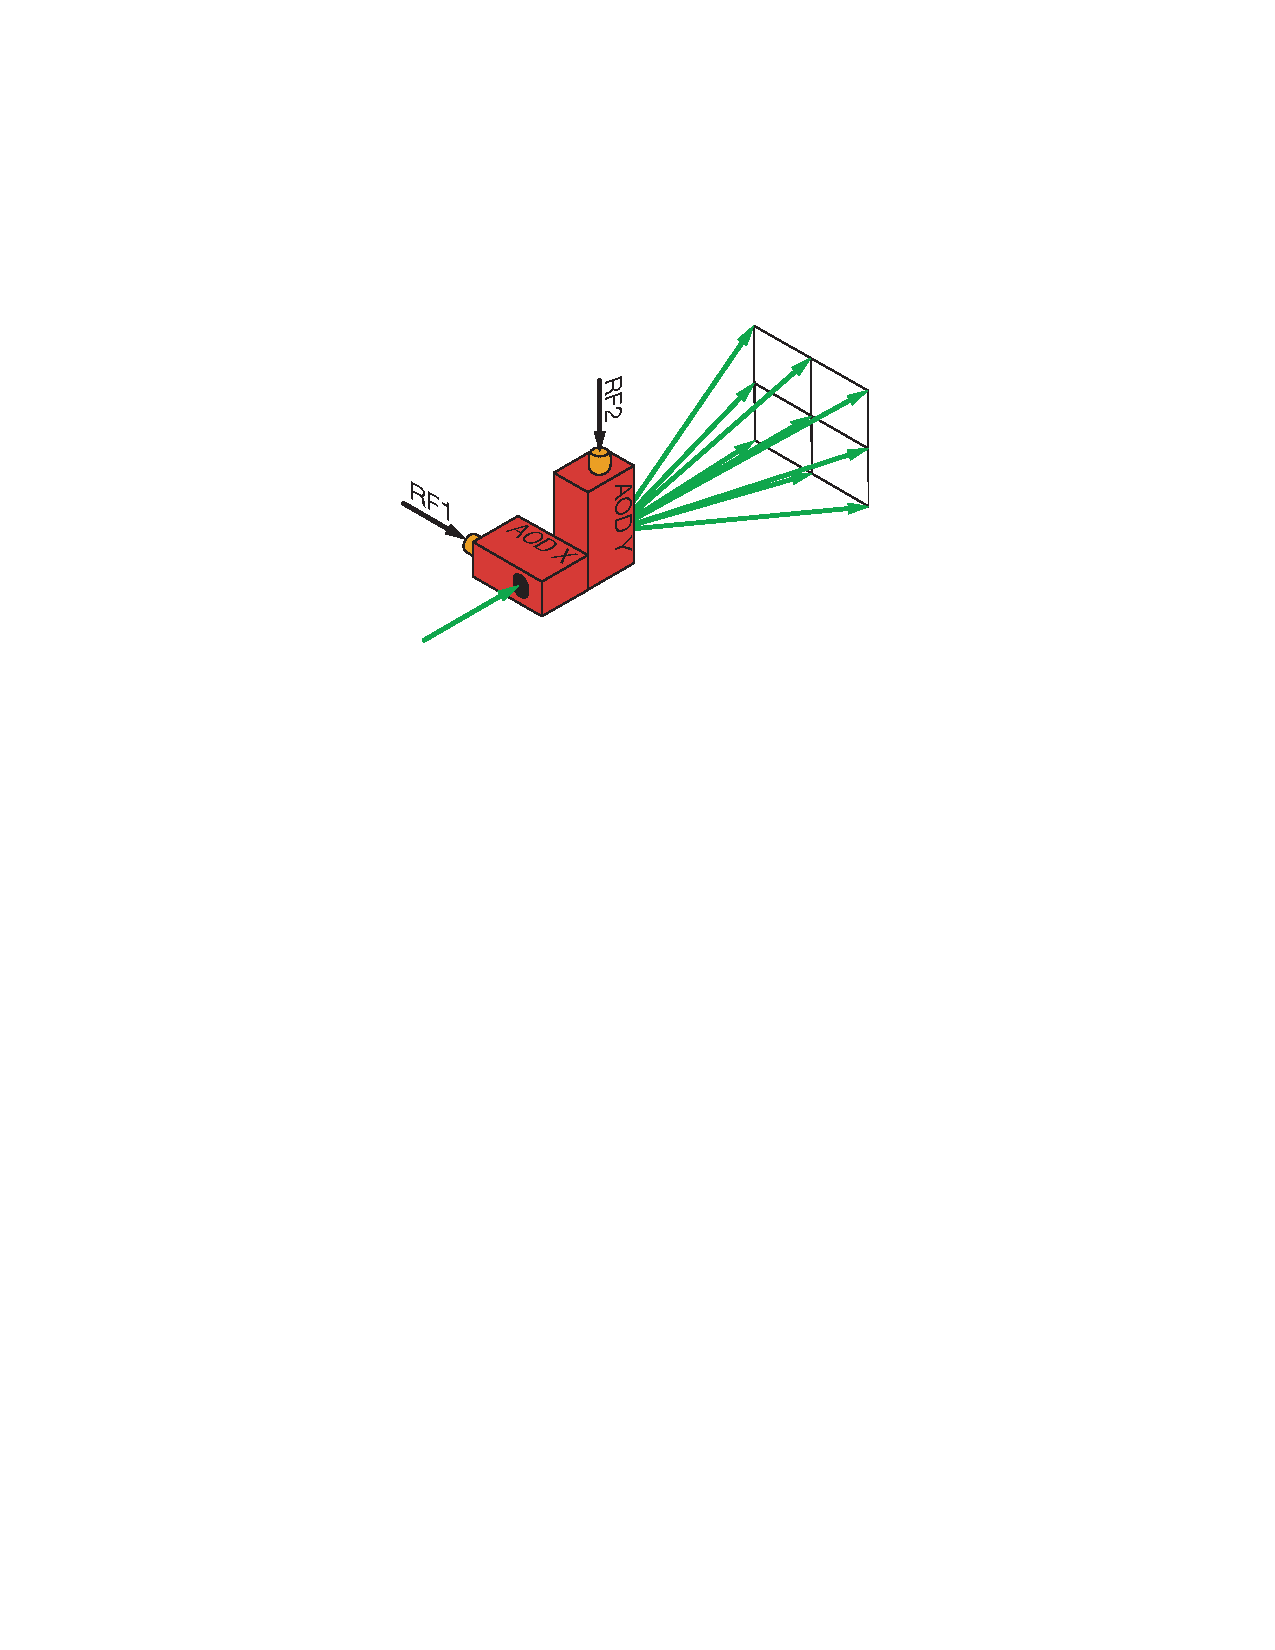
\includegraphics[height=4.25cm]{figures/crossAOD.pdf}
		\caption{}
		\label{fig:CrossAOD}
	\end{subfigure}
	\hfill
	\begin{subfigure}{.59\textwidth}
		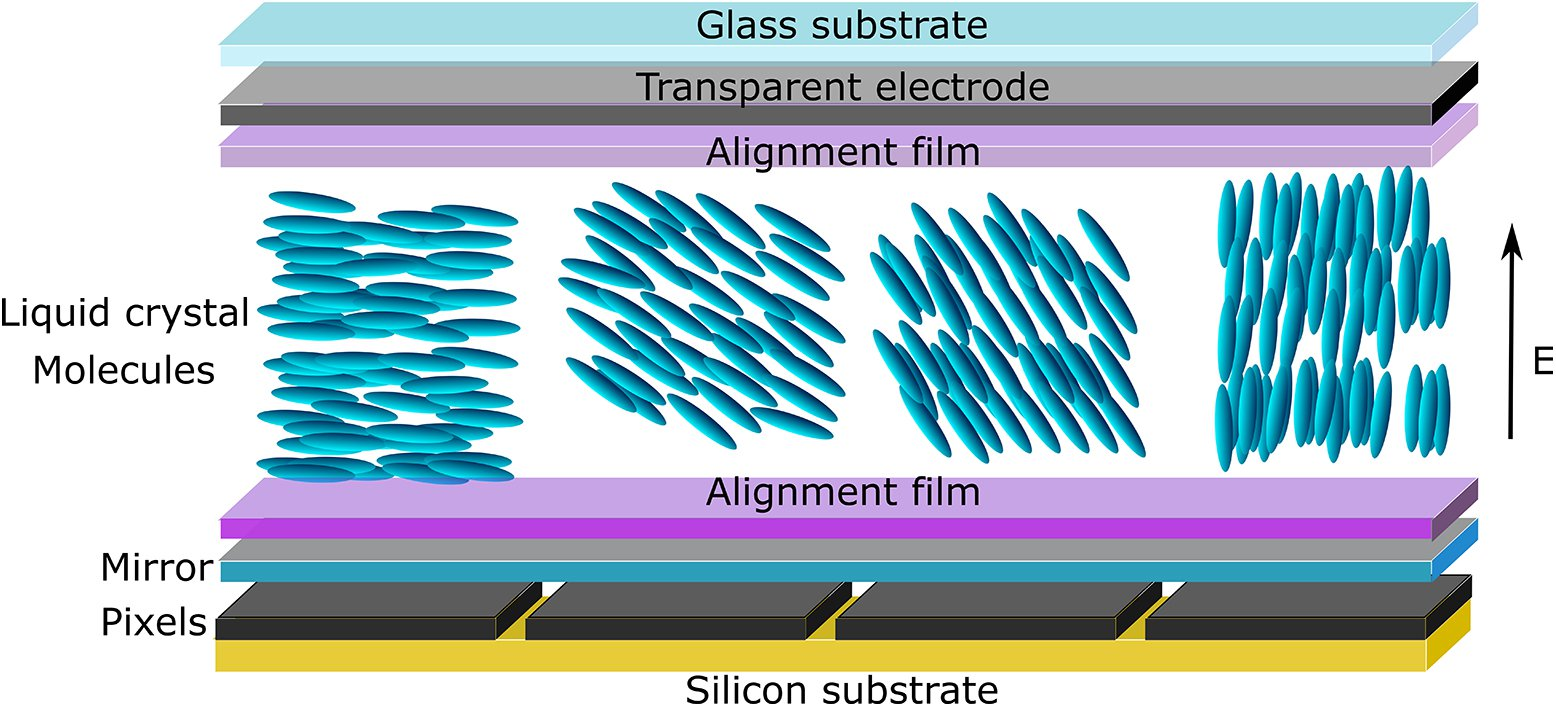
\includegraphics[height=4.25cm]{figures/LCoS.png}
		\caption{}
		\label{fig:LCoS}
	\end{subfigure}
	\caption{\textsf{\textbf{a)}} Two \ac{AOD}s in crossed configuration, used to make a 2D spot array. Figure from \cite{Cooper2018}. 
	\textsf{\textbf{b)}} The orientation of the liquid crystal cells changing as a function of the applied electric field \textit{E}. 
	Figure from \cite{Guzman2017}.}
\end{figure}


\subsection{Diffraction for Spot Arrays}\label{sec:PropagationDerivation}

We will now delve deeper in the diffraction from the SLM hologram, limiting ourselves to producing spot arrays.
First consider the plane of the SLM, denoted in \cref{fig:SLMLens} by the Cartesian coordinates $(x',y',z=0)$. 
If we label the pixels of the SLM with the letter $j$, the phase retardance of this pixel is thus $\phi_j(x'_j,y'_j)$.
Now, consider a laser with intensity distribution $|E_i(x',y')|^2$ reflecting off of the SLM: it will pick up a phase factor such that after the SLM, the field is described as $E_i e^{i\phi(x',y')}$, as shown in \cref{fig:SLMLens}. 
The light field will interfere with itself, until at infinity (or approximately in the focal (Fourier) plane $z'=f$, $z=0$ of a lens) the distribution evolves to $|E_f(x,y,z)|^2$, where $(x,y,z)$ are Cartesian coordinates with the origin in the focus point of the lens as denoted in \cref{fig:SLMLens}.

To see how this works, consider the focal plane or Fourier plane of a lens after the SLM\footnote{In reality, the distance between the SLM and the microscope objective is not the focal length $f$ of the objective, but this will lead to an additional phase factor which can be neglected in practice \cite{Bijnen2013}.}.
In the Fourier plane, the spots in the array will be labeled as $m$, which in general have coordinates $(x_m, y_m, z_m)$ in the Fourier plane, see \cref{fig:SLMgeometry}.
As result of traveling from the pixel $j$ to the trap $m$, under paraxial approximation it can be derived that the light field will experience a phase shift $\Delta_j^m$ \cite{DiLeonardo2007}

\begin{figure}
	\centering
	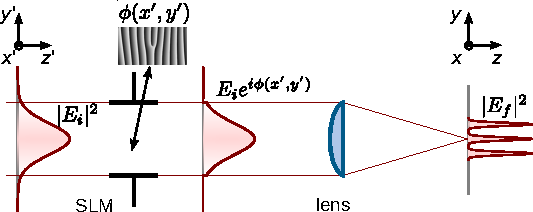
\includegraphics[width = 13cm]{figures/SLMfigure.pdf}
	\caption{Field with intensity distribution $|E_i|^2$ reflects off of the   rectangular SLM, which due to its finite size acts as an aperture in the short-axis direction.
	Also the SLM imprints a phase mask $e^{i\phi(x',y')}$ onto the laser.
	The lens (microscope objective) makes the resulting spot array $|E_f|^2$ in its focal plane.
	Shown on top: two Cartesian coordinate systems in the SLM and focal plane respectively. 
	Figure adapted from \cite{Labuhn2016}.}
	\label{fig:SLMLens}
\end{figure}

\begin{equation}\label{eq:PropagationPhase}
    \Delta_j^m = 
    \frac{2\pi z_m}{\lambdaup f^2} ({x'}_{j}^{2} + {y'}_{j}^{2}) 
    + \frac{2\pi}{\lambdaup f}(x'_j x_m + y'_j y_m).
\end{equation}
The SLM imprints a phase $\phi(x',y') = \phi_j$, leading to a complex electric field vector in the SLM plane for pixel $j$ of

\begin{equation}\label{eq:SLMassumption}
    E_j(x',y') = E_j e^{i \phi_j}.
\end{equation}
In the Fourier plane, the contributions for the different pixels will interfere with each other.
We can find the complex light field $V_m$ (for this section, we will denote the complex light field in the Fourier plane as $V$ similar to \cite{DiLeonardo2007}) for trap $m$ by summing over $N$ pixels $j$ using \cref{eq:PropagationPhase,eq:SLMassumption} \cite{Leseleuc2018}

\begin{equation}\label{eq:DiffractionFormula}
    V_m = e^{i k \left(2 f + z_m\right)}
    \frac{d^2}{i \lambdaup f} \sum_{j=1}^N E_j e^{i(\phi_j - \Delta_j^m)},
\end{equation}
which is essentially using a discrete version of the Fresnel diffraction integral, where $d$ is the pixel pitch of the SLM. 
In \cref{eq:DiffractionFormula}, we can assume uniform illumination of the SLM such that the amplitude is the same everywhere on the SLM or $|E_i| = 1$.
This assumption cannot possibly be valid: we illuminate the SLM with a Gaussian beam from an optical fiber.
However, as will become clear in a moment, the input intensity on the SLM will have no influence on the intensities in the focal plane and this assumption can in fact be used without loss of generality.
In addition, we are really only interested in the intensity $I_m \propto |V|^2$ of each spot, not the phase.
Omitting the pre-factors in \cref{eq:DiffractionFormula} thus yields the dimensionless quantity \cite{DiLeonardo2007}

\begin{equation}\label{eq:Vm}
    V_m \propto \sum_{j} e^{i(\phi_j - \Delta_j^m)}.
\end{equation}
This equation gives the complex field amplitude for spot $m$, given a hologram $\phi_j$.
While \cref{eq:Vm} can be used to compute intensities of 3D spot arrays, an instructive example is setting $z=0$ first \cite{DiLeonardo2007}, for which the quadratic term of \cref{eq:PropagationPhase} disappears.
Substituting the latter term of \cref{eq:PropagationPhase} in \cref{eq:Vm} yields a 2D array of spots with amplitudes 

\begin{equation}\label{eq:2Dcase}
    V_m \propto \sum_j e^{i\phi_j} \exp{\left(
    - i 2\pi \left[
    \frac{x_m}{\lambdaup f} x_j + \frac{y_m}{\lambdaup f} y_j
    \right]
    \right)}.
\end{equation}
This is the 2D \ac{DFT} of the phase array $e^{i\phi_j}$ evaluated at spatial frequencies $x_m/\lambdaup f$ and $y_m/\lambdaup f$ in $x$ and $y$ respectively \cite{Bijnen2015,DiLeonardo2007}, similar to \cref{eq:FraunhoferDiffractionIntegral}.
The DFT is commonly used in signal processing and image analysis and can be easily computed on a computer using \ac{FFT} algorithms. 
FFTs have the advantage that they are way faster to evaluate than the general case of the diffraction formula \cref{eq:Vm}.
In this work, we only use 2D arrays and could in principle use \cref{eq:2Dcase} to speed up calculations.
Because we only computed a small number of holograms, we simply used \cref{eq:Vm}.

\subsection{Computing the Hologram}\label{sec:GSW}

\Cref{eq:Vm} gives the amplitudes of an array of spots given an array of phases $\phi_j$, but we are interested in the reverse problem: what is the hologram $\phi_j$ to be applied, such that we get the spot array of intensities $|V_m|^2$? 
As the equations describing light propagation are time-symmetric, this phase will be the result of $M$ coherent light sources radiating with $w_m e^{i \theta_m}$, picking up a propagation phase described by \cref{eq:PropagationPhase}, leading to a complex amplitude in the \ac{SLM} plane of \cite{Leseleuc2018,DiLeonardo2007}

\begin{equation}\label{eq:InterferencePattern}
    E_j (x',y') = \sum_m w_m \exp{
    i\left(\Delta_j^m + \theta_j\right)
    }.
\end{equation}
But producing the light field in \cref{eq:InterferencePattern} requires doing phase as well as amplitude modulation, which is not possible: the SLM can only do phase modulation.
So in this step in the algorithm, we take the argument of  \cref{eq:InterferencePattern} yielding the following hologram

\begin{equation}\label{eq:Argument}
    \phi_j = \text{arg}\left\{
     \sum_m w_m \exp{
    i\left(\Delta_j^m + \theta_j\right)
    }
    \right\}.
\end{equation}
But the lack of amplitude modulation leads to a loss of information, and the hologram produced by \cref{eq:Argument} will not produce the result we seek.
The solution to this problem was solved by \cite{Gerschberg1972}, who pioneered the \ac{IFTA} algorithm or Gerschberg-Saxton algorithm.
The core idea of the algorithm is to virtually propagate light between SLM and focal planes, using (inverse) Fourier transforms like \cref{eq:2Dcase}.
In each propagation step, the hologram in the SLM plane and the computed pattern in the Fourier plane are updated in an iterative fashion, until a solution (the desired pattern and the corresponding hologram) are obtained.
For a more detailed description of an implementation of IFTA algorithms the reader is referred to \cite{Bijnen2015,Bijnen2013}.
A key advantage of using these kinds of algorithms is from \cref{eq:Vm}: each pixel contributes to each individual spot.
As a result, using this algorithm, no knowledge about the laser input field is needed, which can be hard to determine exactly in practice.

For 3D spot arrays, Fourier transforms cannot be used, and the algorithm was extended using \cref{eq:Vm,eq:Argument} by \cite{DiLeonardo2007}. 
This algorithm is called the \ac{GSW} algorithm, which is sketched in \cref{fig:GSWalgorithm}.

\begin{figure}
	\centering
	\begin{subfigure}{.56\textwidth}
		\centering
		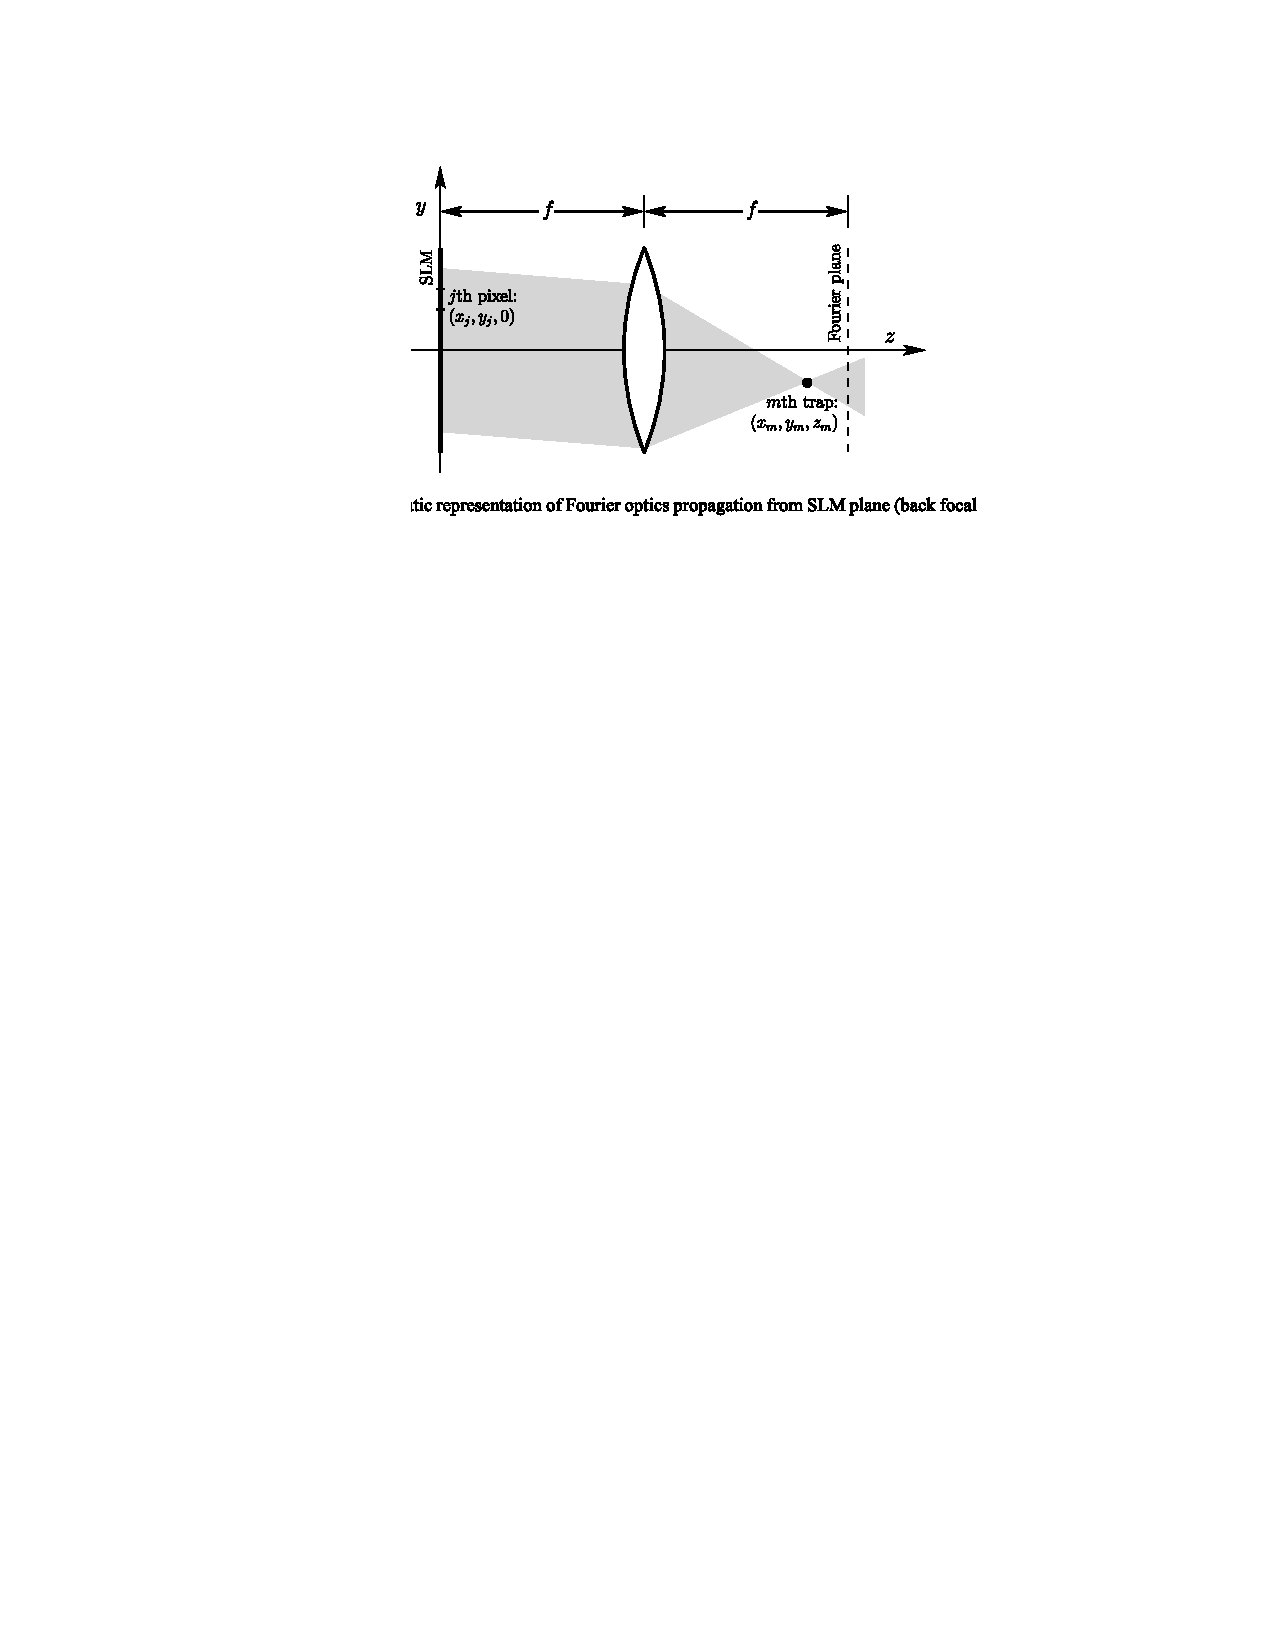
\includegraphics[height=5.3cm]{figures/SLMgeometry.pdf}
		\caption{}
		\label{fig:SLMgeometry}
	\end{subfigure}
	\begin{subfigure}{.43\textwidth}
		\centering
		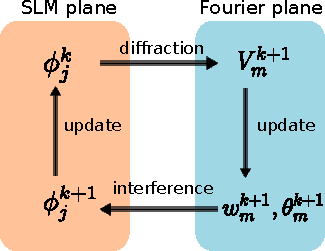
\includegraphics[height=5.3cm]{figures/WeightedGerschbergSaxton.pdf}
		\caption{}
		\label{fig:GSWalgorithm}
	\end{subfigure}
	\caption{\textsf{\textbf{a)}} SLM plane with phases $\phi_j(x,',y',0)$ for pixel $j$, as well as the focal plane or Fourier plane with trap coordinates for trap $m$ of $(x_m,y_m,z_m)$. 
		Figure from \cite{DiLeonardo2007}. 
		\textsf{\textbf{b)}} The \ac{GSW} algorithm visualized.
		The light field is virtually propagated between the SLM and focal planes using \cref{eq:Vm,eq:Argument}, continuously updating the weight factors $w_m^k$ as well as the hologram $\phi_m^k$.}
	\label{fig:GerschbergSaxton}
\end{figure}

\subsubsection*{The GSW Algorithm}

\begin{enumerate}
    \item Starting with hologram $\phi_j^k$, the diffraction equation \cref{eq:Vm} is used to compute the complex amplitudes of the spot array $V_m^{k+1}$. 
    
    \item From the amplitudes $V_m^{k+1}$, the new weight factors $w_m^{k+1}$ and phases $\theta_m^{k+1}$ are computed.
    
    \item From the weight factors $w_m^{k+1}$ and phases $\theta_m^{k+1}$, the interference equation \cref{eq:Argument} tells us what the resulting phase on the SLM pixel array $\phi_j^{k+1}$ would be, by assuming an array of point sources radiating with amplitudes $w_m$ and phases $\theta_m$.
    
    \item The iteration counter $k$ is increased to $k+1$, the hologram is updated and the steps above are repeated.
\end{enumerate}
As a initial ansatz for the algorithm, we start with a hologram computed by using \cref{eq:Argument} for an array of traps of uniform intensities $w_m^{k=0} = 1$ and random phases $\theta_m^{k=0} \in (0, 2\pi)$.
After each iteration, the diffraction efficiency $e$ (the real part of the complex interference pattern) and the uniformity $u$ of the array $V_m$ should increase until convergence, yielding a set of target amplitudes $V_m$ as well as a hologram $\phi_j$ that produces this set of amplitudes.
The definitions of the diffraction efficiency $e$ and uniformity $u$ are 

\begin{equation}\label{eq:EfficiencyUniformity}
    e = \frac{1}{M}\sum_m |V_m|^2, 
    \quad 
    u = 1-\frac{\text{max}(|V_m|^2)-\text{min}(|V_m|^2)}{\text{max}(|V_m|^2)+\text{min}(|V_m|^2)},
\end{equation}
and are evaluated after each iteration $k$. 
The algorithm stops if the user-defined minimum criteria for diffraction efficiency or uniformity are met.

\subsubsection*{Implementation}

The algorithm was implemented in Python by Ivo Knottnerus as part of his PhD research.
Because the SLM has $\sim 2$ million pixels, converting to and from the SLM plane, so performing equations \cref{eq:Vm,eq:Argument}, can be time consuming depending on the desired pattern.
Therefore, these computations are performed on a graphics card using the \textit{PyOpenCL} library. 
After a couple tens of iteration steps, we typically see the diffraction efficiency converging to $e \sim 0.92$.
The theoretically computed uniformity will continue to increase indefinitely, but is typically already on the order $u \sim 0.999$ after $\sim 10^2$ iterations, where larger arrays take more iterations to reach the same uniformity.
A typical hologram using the algorithm is shown in \ref{fig:SLMphase}a as well as \ref{fig:HologramPattern}.


\section{Operating the SLM}\label{sec:SLMoperatoin}

Because the SLM used previously in our group suffered from amplitude modulation \cite{Bijnen2015,Dijk2012}, an unwanted effect, we purchased a newer model SLM. Specifically, the Meadowlark E-series 1920 x 1200 SLM.
A few specifications of the device are presented in \cref{table:SLMspecs}.
In the next section, we will elaborate upon some other practical considerations that have to be taken into account in operating the SLM.

\begin{table}[h]
    \centering
    \caption{Key specifications of the Meadowlark SLM.}
    \label{table:SLMspecs}
    \begin{tabular}{l | l}
        \textbf{Specification}              & \textbf{Value}        \\ \hline 
        Array size                          & 15.4 x 9.6 mm         \\ \hline
        Resolution                          & 1920 x 1200 pixels    \\ \hline
        Bit depth                           & 8 bit                 \\ \hline
        Diffraction efficiency (785 nm)  & 76-79\%   
    \end{tabular}
\end{table}


\subsection{Electro-Optical Response}

The refractive index $\Delta n(V)$ and therefore the light retardation $\phi(V)$ of \cref{eq:ElectroOpticResponse} are not necessarily linear as a function of the applied voltage.
Thus it is needed to calibrate the electro-optic response of the \ac{SLM}, which equates to measuring the retardation $\phi$ as a function of the applied voltage $V$. 
This calibration serves two purposes:

\begin{enumerate}
    \itemsep=0pt
    
    \item Ensure the minimum to the maximum phase retardation corresponds to a $2\pi$ (one wave) phase retardation.
    
    \item Linearize this electro-optical response curve. 
\end{enumerate}
The calibration has to be performed because each individual SLM has a slightly different electro-optical response. 
Furthermore, it is wavelength specific, which is why we performed it for the wavelength relevant for Rb experiments at 820 nm. 
Measuring the electro-optical response directly is impossible because the light field oscillates with frequencies in the THz regime.
There are a variety of methods to measure it indirectly for a phase-only \ac{SLM}, however \cite{Li2019}.
We chose the diffractive calibration method, originally proposed by \cite{Zhang1994}.
The method works by applying a variety of Ronchi gratings onto the SLM, see \cref{fig:LUTCalibrationSetup}.
This is a pattern consisting of $M$ periods of width $w=8$ pixels in the horizontal direction and a vertical height $H$ of gray values $L$ alternating between $L=L_1$ and $L=L_2=0$.
Gray values are 8 bit numbers representing the degree of modulation where 0 (black) means no modulation or $V=0$ while 255 (white) is maximum modulation: $V=5$V. As an example, we first consider a Ronchi grating with ones period $M=1$, shown in \cref{fig:OneGrating}.

\begin{figure}[h]
    \centering
    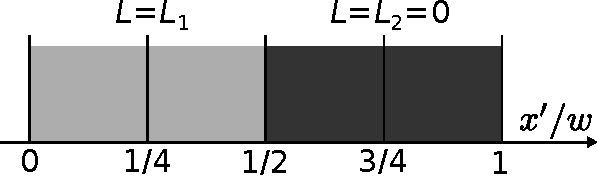
\includegraphics[width=0.42\textwidth]{figures/OneGrating.pdf}
    \caption{Ronchi grating for a single grating $M=1$ as well as $L_2=0$.}
    \label{fig:OneGrating}
\end{figure}

\noindent Assuming amplitude modulation between different gray levels is negligible (a fair assumption for phase-only SLMs), after applying the Ronchi graing of \cref{fig:OneGrating} the electric field just after the SLM will be

\begin{equation}\label{eq:Single}
    f(x,y) = e^{i\phi(L_1)} \operatorname{rect} \left\{ 
    \frac{x'-w/4}{w/2}\right\} +
    \operatorname{rect}\left\{ \frac{x'-3w/4}{w/2}\right\}.
\end{equation}
In \cref{eq:Single} $\operatorname{rect}\{(x'-a)/b\}$ is the rectangular function, which is unity for a width $b$ centered around $x'=a$ and zero elsewhere.
In the case of the single grating, $\{a=1/4, 3/4\}$ and $b=w/2$.
For $M>1$, this pattern is simply repeated an additional $M-1$ times \cite{Zhang1994}

\begin{equation}\label{eq:FieldAfterSLM}
    f(x,y) = \sum_{m=0}^{M-1} \left[
    e^{i \phi(L_1)} \operatorname{rect}\left\{\frac{x'-m w - w/4}{w/2}\right\} + 
    e^{i \phi(L_2)}\operatorname{rect}\left\{\frac{x'- m w - 3 w/4}{w/2}\right\}
    \right].
\end{equation}

\begin{figure}
	\begin{subfigure}{.51\linewidth}
		\flushleft
		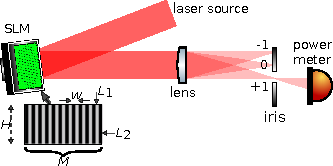
\includegraphics[height=5cm]{figures/LUTcalibrationSetup.pdf}
		\caption{}
		\label{fig:LUTCalibrationSetup}
	\end{subfigure}
	\hfill
	\begin{subfigure}{.48\linewidth}
		\flushright
		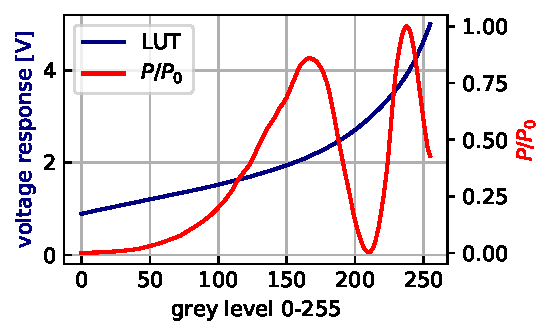
\includegraphics[height=5cm]{figures/LUTplot.pdf}
		\caption{}
		\label{fig:LUTcalibration}
	\end{subfigure}
	\caption{\textsf{\textbf{a)}} Ronchi grating on the SLM with gray values $L_1$ and $L_2$. 
	The diffraction orders are separated using a $f=400$ mm lens. 
	Other diffraction orders than $+1$ are blocked using an iris. 
	\textsf{\textbf{b)}} Normalized power in the first order as a (\textcolor{red}{red}) and the fitted voltage response (\textcolor{blue}{blue}) as a function of the applied gray level $L_1 \in (0-255)$.}
\end{figure}

\noindent According to Fourier optics, if we place a lens after the SLM, the field in the \textit{Fourier} plane of the lens is the 2D spatial Fourier transform of the field after the SLM, as derived in \cref{eq:FraunhoferDiffractionIntegral} as well as in \cref{eq:2Dcase}.
The field is thus for $y=0$ (we separate the different orders in the $x$-direction around $y=0$) proportional to the spatial Fourier transform $F = \mathcal{F}(f)$, and the intensity $I\propto |F|^2|$ as \cite{Zhang1994}

\begin{equation}\label{eq:FourierIntensity}
    |F(p,0)|^2\propto
    \frac{M^2 w^2}{2}\operatorname{sinc}^2\left(\frac{M p w}{2}\right) \times
    \frac{1 + \cos{\left[\phi(L)+p w/2\right]}}{\cos^2(p w/4)}.
\end{equation}
In \cref{eq:FourierIntensity} $p=2\pi x/\lambdaup f$ is the Fourier transformed spatial coordinate. The intensity in the first order ($p=\pm 2\pi/w$) is

\begin{equation}\label{eq:IntensityFirstOrder}
    I_1(\phi(L_1)) \propto
    \frac{w^2}{\pi^2} \left[ 
    1-\cos{\phi(L_1)}
    \right],
\end{equation}
which is a useful expression as it gives a relation between the power in the first order (which we can measure) as a function of the applied gray level $L_1$.
Experimentally, we load a sequence of Ronchi gratings onto the SLM, looping $L_1$ from the minimum $L_1=0$ to the maximum gray value $L_1=255$, while keeping $L_2 =0$ the whole time.
For our 8-bit SLM, this amounts to looping over 255 gray values, which we did with the help of an edited \textit{labVIEW} script from the manufacturer.
For each hologram, separate the multiple diffraction orders using a $f=400$ mm lens (such that the spacing between the various orders is sufficient) and an aperture and record the power in the first order using a power meter.

The results are shown in \cref{fig:LUTcalibration}. 
In red we show the normalized power in the first order $P/P_0$ as a function of the applied gray level $L_1$, where $P_0$ is the maximum recorded power in the first order.
In blue we show the result of fitting the data using a program provided by the manufacturer.
This is also called the gamma curve or \ac{LUT}.
The LUT is what the SLM uses to connect the 8-bit gray level to 10-bit voltage levels in a linear fashion, ensuring the gray level range corresponds to $2\pi$ phase retardation.
As can be seen from \cref{fig:LUTcalibration}, the obtained LUT is rather non-linear, meaning the electro-optical response for a linear LUT would be non-linear, as expected. 

Using our newly acquired LUT, we measured a diffraction efficiency in agreement with the specifications in \cref{table:SLMspecs}. 
The exact diffraction efficiency depends on the 'smoothness' of the pattern applied to the SLM: because of the pixelated nature the SLM can only approximate continuous patterns. 
More rapidly-varying patterns equal lower diffraction efficiency \cite{Labuhn2016}.

\subsection{Rectangular SLM Aperture}\label{subsec:ApertureSize}

In order to make use of the maximum amount of degrees of freedom (pixels) the SLM has to offer, the active area should be fully illuminated.
However, because the incident beam is described by a Gaussian, this will lead to power loss as a result of light falling outside of the chip area.
The ideal incident waist size is thus a compromise between power efficiency on the one and amount of pixels used on the other hand.
We estimate this power loss by reflecting a Gaussian beam $G(x,y)$ having waist $w(z)$ and power $P_0$ off of a rectangular aperture of dimensions $(2S_x, 2S_y)$ where $S_{x,y}$ are the semi-widths of the aperture, see \cref{fig:Rectangular}.
\begin{figure}[h]
    \centering
    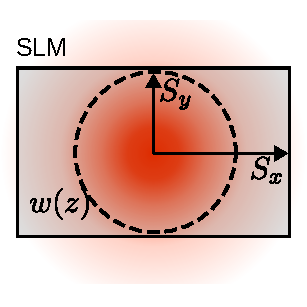
\includegraphics[width=0.31\textwidth]{figures/RectangularAperture.pdf}
    \caption{Laser beam with waist $w(z)$ reflecting off the SLM with rectangular semi-widths $S_x$ and $S_y$.}
    \label{fig:Rectangular}
\end{figure}

\noindent The relative power transmission $P/P_0$ can be found by integrating the intensity of the beam \cref{eq:GaussianBeamIntensity} in Cartesian coordinates over the aperture

\begin{equation}\label{eq:RectAperturePower}
	\frac{P}{P_0} =
	\iint G(x,y) dA=
	\text{erf}\left(\frac{\sqrt{2}S_x}{w(z)}\right) \text{erf}\left(\frac{\sqrt{2}S_y}{w(z)}\right).
\end{equation}
If we use a beam with $1/e^2$ radius equal to the short semi-width SLM and using the aspect ratio from \cref{table:SLMspecs}, the power transmission is $\sim 95$\%.
So we barely lose any power, while still using as much pixels as possible.
The pixels outside of the beam waist radius contribute less, but are unused when focusing the SLM beam onto the circular objective pupil (see \cref{sec:Demagnification}).
To obtain this waist, we direct the beam on the SLM from the Schäfter fiber collimator (\cref{sec:MeasuringTweezer}).
This collimator yields a beam with waist $w(z)$ mm, about the size of the short semi-width $S_y = 4.8$ mm of the rectangular SLM.




\subsection{Diffraction Orders}\label{subsec:Diffraction}

Because the SLM is a periodic structure with constant pixel pitch $d$, multiple diffraction orders will reflect off of the device, lowering the amount of power in the main diffraction order.
The power in the higher diffraction orders is unused. 

\begin{figure}
	\centering
	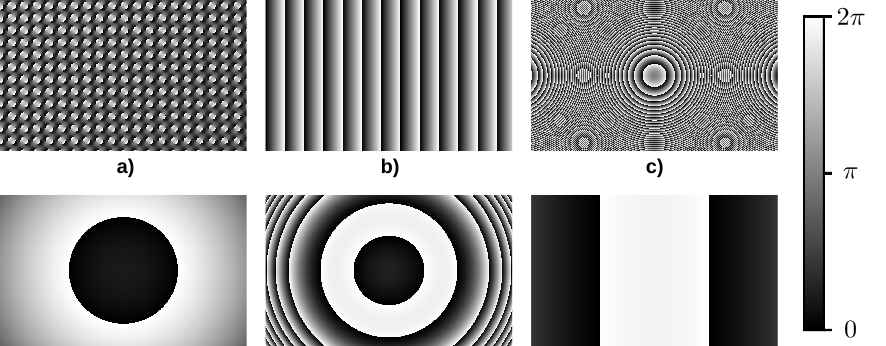
\includegraphics[width=\textwidth]{figures/hologram.png}
	\caption{
		Total phase mask applied on the SLM: \textsf{\textbf{a)}} Hologram obtained from the \ac{GSW} algorithm to generate the spot array.
		\textsf{\textbf{b)}} Lens phase applied to use the SLM as the first lens of a telescope with magnification $M=0.42$.
		\textsf{\textbf{c)}} Optical flatness correction pattern as provided by the manufacturer.
		\textsf{\textbf{d)}} Linear phase ramp, used to move the diffraction pattern away from the optical axis (zoomed in).
		\textsf{\textbf{e)}} Aberration correction phase applied onto the SLM, which is a fourth-order polynomial in the distance from the center.
		\textsf{\textbf{f)}} Cylindrical lens phase to account for aberration introduced by the SLM itself.
	}
	\label{fig:SLMphase}
\end{figure}

In addition, there will always be a fraction of light that is not modulated.
This light originates from reflection off of the glass cover on top of the birefringence layer or from the unused space between the pixels and is focused to a single spot in the glass cell by the objective \cite{Bijnen2013}.
To get rid of this undesired light, typically a linear phase is superimposed on top of the hologram (tilt aberration) which translates the desired pattern away from the undiffracted light.
The type of linear phase used is shown in \cref{fig:SLMphase}b, as well as the hologram producing the spot array in \cref{fig:SLMphase}a.
The sum of the total hologram is computed modulo $2\pi$, which equals exactly one wave retardation.
After translating away the diffraction pattern from the zeroth order beam, the latter can be spatially filtered out in an intermediary focus point and an iris. 
It is worth noting that this method comes at the cost of a slightly lower diffraction efficiency, because the phase ramp applied can only be approximated by the pixelated SLM.

\subsection{Beam size decrease}\label{sec:Demagnification}

To prevent excess loss of power, the $w = 4.8$ mm beam needs to be adapted to the $R = 2.0$ mm radius of the microscope objective. 
Thus the beam should be magnified by a factor $M=0.42$ (demagnified).
This is commonly done using a Keplerian telescope using two lenses $f_1$ and $f_2$ as shown in \ref{fig:SLMbeampath}a.
Moreover, apart from adapting the beam size, the telescope serves two more functions:

\begin{itemize}
    \item Conjugate the SLM plane and objective aperture planes.
    This means that for any arbitrary angular pattern applied by the SLM, the light field will remain centered on the circular aperture of the objective \cite{Nogrette2014}. 
    
    \item Allow for spatial filtering: the intensity profile is only produced in the focal plane of a lens (\cref{sec:InFocus}).
    Thus to remove unwanted light from unwanted diffraction orders, an intermediary focus plane is needed which is provided in any case when using a Keplerian telescope.
\end{itemize}
To accommodate room for the objective holder, (dichroic) mirrors, a polarizing beam splitter cube leave room for additional optics in the future, we estimate from a CAD drawing we need $\sim 45$ cm of room between the last relay lens of the telescope and the objective. 
Using a Keplerian telescope, this distance will be equal to $f_2$ (\cref{fig:SLMbeampath}).
Also knowing that $f_1=f_2/M$ and the total length of the telescope is $2f_1+2f_2$, this is already $\sim 305$ cm of beam path on the optical table. 
To reduce this, we borrowed a trick from our collaborators at the University of Amsterdam, where we use the SLM as the first lens of the system with focal length $f_s$ in conjunction with another relay lens $f_r$ (see \cref{fig:SLMbeampath}, to not confuse ourselves with $f_1$ and $f_2$ of the equivalent Keplerian telescope we renamed the variables). 
In terms of the ABCD matrix formalism, the transfer matrix $\mathbf{M}$ for the system in \cref{fig:SLMbeampath}b is

\begin{figure}
	\centering
	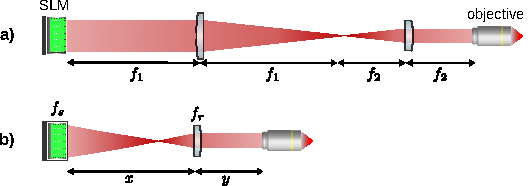
\includegraphics[width=0.95\textwidth]{figures/beampathSLM.pdf}
	\caption{\textsf{\textbf{a)}}: Keplerian telescope with total length $2f_1+2f_2$. \textsf{\textbf{b)}} Using the SLM as a lens $f_s$ in conjunction with a relay lens $f_r$, the total beam path has length $x+y$. In the latter case, $y>f_r$.}
	\label{fig:SLMbeampath}
\end{figure}

\begin{equation}\label{ABCD}
	\mathbf{M}=
	\begin{pmatrix}
		1 & y \\
		0 & 1
	\end{pmatrix}
	%
	\begin{pmatrix}
		1 & 0 \\
		-1/f_r & 1
	\end{pmatrix}
	%
	\begin{pmatrix}
		1 & x \\
		0 & 1
	\end{pmatrix}
	%
	\begin{pmatrix}
		1 & 0 \\
		-1/f_s & 1
	\end{pmatrix}.
\end{equation}
Substituting $x= f_r(1+f_s/f_r)$ and $y=f_r(1+f_r/f_s)$, \cref{ABCD} reduces to

\begin{equation}
	\mathbf{M}=
	\begin{pmatrix}
		-f_s/f_r & 0\\
		0 & -f_r/f_s
	\end{pmatrix}.
\end{equation}
This is the ABCD matrix for a beam expander. The total length is $x+y = 102 + 42.5 = 145$ cm for $f_r = 300$ mm and $f_r/f_s=0.42$, which is significantly shorter than when using a conventional telescope.

We will now explain how we computed the hologram to produce a focal length $f_s = 30 / 0.42 = 69$ cm on the SLM.
The Fresnel lens hologram is essentially to a defocus 'aberration'.
It is common to quantify aberrations in terms of Zernike's functions, a set of polynomials orthogonal on the unit disk. 
The SLM is not circular, but the part of the SLM that is conjugated with the microscope objective is, so we consider the SLM as a circle for now, with the radius equal to the short semi-width $S_y$.
Now, the coordinates on the unit disk can be denoted as $\rho = r/S_y$ and $\theta \in (0, 2\pi)$, such that the wavefront $\phi(\rho,\theta)$ can be expanded in terms $R_n^m(\rho)\cos{m\theta}$ and $R_n^m\sin{m\theta}$ where 

\begin{equation}\label{eq:ZernikeRadial}
    R_{n}^{m}(\rho)=
    \sum_{s=0}^{(n-m) / 2}
    \frac{(-1)^{s}(n-s) !}{s !\left((n+m)/2-s\right) !\left((n-m)/2-s\right) !} \rho^{n-2 s}
\end{equation}
is the radial Zernike polynomial set \cite{Mahajan94}.
In this work, we only consider radially symmetric polynomials so we only use \cref{eq:ZernikeRadial}, without the $\theta$ dependence.
The defocus aberration in terms of the defocus coefficient $S_2$ is $S_2 R_2^2 = S_2\rho^2$.
We want to find this coefficient $S_2$, which we do by equating the defocus aberration to the exponent of an equivalent Fresnel lens with focus $f_s$ (\cref{eq:Transfer}):

\begin{equation}
    \frac{i k }{2 f_{s}}r'^2=i 2\pi S_2 \rho^2, \quad \rho = \frac{r'}{S_y}.
\end{equation}
Solving for $S_2$ yields $S_0 = k S_y^2/(4\pi f_s)= 20.4$ for $f_{s} = 69$ cm and  $S_y = 4.8$ mm.
The Fresnel lens hologram used on the SLM to make the beam expander (which is a quadratic polynomial) is shown in \ref{fig:SLMbeampath}c.


\subsection{Optical Flatness}\label{subsec:Flatness}

Because of manufacturing imperfections, the SLM chip will not be perfectly flat on the scale of the wavelength of the light used. 
The exact shape of the chip area is slightly different between individual SLM units.
The flatness of our chip was measured by manufacturer Meadowlark to have a RMS flatness of $\sim 0.18\lambdaup$ (785 nm).
The shape of the flatness was measured as well and provided to us by the manufacturer, so we can correct for it by subtracting a phase mask corresponding to the same non-flatness.
This mask is shown in \ref{fig:SLMphase}c.


\subsection{Aberration Correction}\label{subsec:AberrationCorrection}

Now that the SLM has been introduced, we will explain more thoroughly how exactly we corrected for spherical aberration as introduced by the incorrect glass thickness (\cref{sec:Tweezer3D}).
We left off at \cref{eq:SphericalFocus}.
For paraxial rays ($\alpha_0 \rightarrow 0$), \cref{eq:SphericalFocus} reduces to $d(1-1/n)$. 
Subtracting this paraxial result from the case for general ray angles, which may contain large angles from \cref{eq:SphericalFocus} and Taylor expanding up to fourth order in $\alpha_0$ yields the difference in focus shift between the general and paraxial case of \cite{Iwaniuk2011}

\begin{equation}\label{eq:FocusDifference}
    \delta f(\alpha_0,n,d)= \Delta f_{\text{general}} - \Delta f_{\text{paraxial}} \approx
    d\left(\frac{n^2-1}{2n^3}\right)\alpha_0^2 - d\left(\frac{9-10n^2+n^4}{24n^5}\right)\alpha_0^4+\mathcal{O}(\alpha_0^6).
\end{equation}
Multiplying \cref{eq:FocusDifference} with $(n-1)/\lambdaup$ converts the path length difference to a phase difference $\phi(\theta)/2\pi$.
This phase difference is plotted in \cref{fig:AberrationTerm}a as a function of the incident angle $\alpha_0$.
This is a very substantial error, most likely not enough to fully correct using the SLM. 
Luckily, we use a microscope objective that is already corrected for $d_o=3.5$ mm of $n_o=1.510$. 
We subtract this contribution from \cref{eq:FocusDifference}, which was filled in for $d_g=4.0$ mm of $n_g=1.453$, leaving only a small error in the refractive index and thickness mismatch.
Again, we multiply with $(n-1)/\lambdaup$, finding the mismatch in the correction in terms of waves $\delta \phi$

\begin{equation}\label{eq:Mismatch}
    \delta \phi(\alpha_0)=
    \frac{n_o-1}{\lambdaup}\cdot
    \left[\delta f(\alpha_0,d_g,n_g)-\delta f(\alpha_0,d_o,n_o)\right].
\end{equation}
The result of \cref{eq:Mismatch} is plotted in \cref{fig:AberrationTerm}b.
\begin{figure}
    \centering
    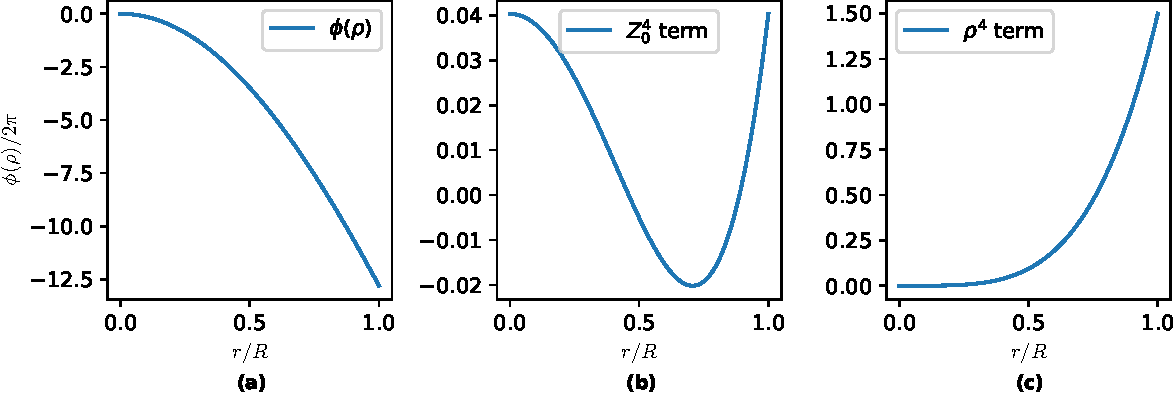
\includegraphics[width=\textwidth]{figures/SphericalAberrationTerms.pdf}
    \caption{
    \textsf{\textbf{a)}} Total phase error from \cref{eq:FocusDifference} without subtracting the correction of the Mitutoyo objective.
    \textsf{\textbf{b)}} Aberration remaining after subtracting the Mituotoyo correction.
    \textsf{\textbf{c)}} Only the $Z_0^4$ (spherical aberration) term. This we actually apply on the SLM.
    }
    \label{fig:AberrationTerm}
\end{figure}
We still need to convert the angular dependence on a radial dependence in the objective plane. 
Because the SLM plane is conjugated with the objective plane, this is equivalent to a radial dependence on the SLM. We convert from angles to radial distance in the objective plane $r'$ as

\begin{equation}\label{eq:RadialCoordinate}
    \alpha_0 = \operatorname{arcsin}\left(\frac{r'\text{NA}}{R}\right)
    =\operatorname{arcsin}\left(\rho \text{NA}\right).
\end{equation}
Here, we again used $\rho=r'/R$, hinting at the use of Zernike's polynomials again.
In terms of Zernike functions.
Substituting \cref{eq:RadialCoordinate} in the \cref{eq:Mismatch} and expanding in Zernike polynomials only the following terms remain:

\begin{equation}
    \delta \phi(\rho) = S_0 R_0^0(\rho) + S_2 R_2^2(\rho) + S_4 R_4^0(\rho).
\end{equation}
The first term $S_0$ is simply a constant having no effect on the diffraction and can thus be omitted. 
The $S_2$ term corresponds to defocus, which we already used in \cref{sec:Demagnification}.
In this case , it is the result of the changing focus distance of placing additional glass in the beam path.
We fix this term by adjusting the focus of the objective and can thus be discarded as well.
This leaves only the $Z_4^0 = 1 - 6 \rho^2 + 6 \rho^4$ term, which we plotted for $\rho=r'/R$ in \cref{fig:AberrationTerm}c.
This primary spherical aberration was applied onto the SLM, its corresponding hologram is shown in \cref{fig:SLMphase}e.


Even after the spherical aberration correction, we still noted unsatisfactory performance in the axial direction as discussed in \cref{sec:Tweezer3D}. 
We think this is due to the lens phase on the SLM (\cref{fig:SLMLens}b): because the laser reflects off of the device, it effectively travels through a biconvex lens under this same angle (astigmatism aberration). 
This can cause the focus position to change slightly between $x$ and $y$, which would explain the increased Rayleigh range measured. 
We corrected for this by applying an additional lens phase only in the horizontal direction as shown in \cref{fig:SLMphase}f.


\section{Characterizing Tweezer Arrays}\label{sec:ArraysResults}

Using the \ac{GSW} algorithm implemented in Python code by Ivo Knottnerus, we generated holograms corresponding to $n \times n \times 1$ pixels in the $x$, $y$ and $z$-directions respectively, where $n = 1,2,\ldots 10$ (larger arrays are possibly, but cannot be fully imaged onto the CCD camera used because of the limited field of view in conjunction with the 0.85 NA objective). 
The algorithm was run until the uniformity $u$ reached 0.999. 
A typical hologram that was obtained is shown in \cref{fig:SLMphase}a.
Here, an example for a $7 \times 7$ array was used. 
In \cref{fig:SLMphase}b, the simulated diffraction pattern from this phase mask is shown. 
The units in this Fourier plane are so-called focal units, which are the Fourier transformed coordinates \cite{Bijnen2015}



\begin{figure}
    \centering
    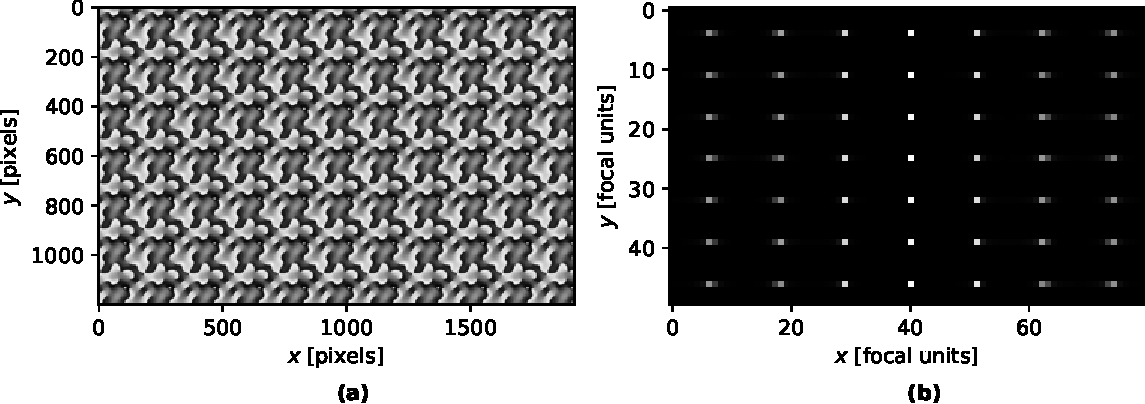
\includegraphics[width=\textwidth]{figures/MaskAndComputedPattern.pdf}
    \caption{\textsf{\textbf{a)}} Hologram computed by the \ac{GSW} algorithm to compute a $7\times7$ spot array.
    \textsf{\textbf{b)}} Diffraction pattern as computed from the algorithm using the hologram in \textsf{\textbf{(a)}} in focal units (\cref{eq:FocalUnit}.}
    \label{fig:HologramPattern}
\end{figure}

\begin{equation}\label{eq:FocalUnit}
    \Delta x \times \Delta y = \frac{\lambdaup f}{S_x}\times \frac{\lambdaup f}{S_y},
\end{equation}
where $S_x = 7.7$ mm and $S_y = 4.8$ mm are the semi-widths of the rectangular SLM aperture in $x$ and $y$ directions respectively.
Multiplying the spacing in focal units in \cref{fig:HologramPattern} with the definitions in \cref{eq:FocalUnit} will lead to a uniform spacing of $\sim 5$ $\mu$m in the Fourier plane. 
Because of non-integer spacing in focal units of the target pattern and the pixelated nature of the array of focal units in \ref{fig:HologramPattern}b, for some spots the peaks are spread out over multiple pixels, but this has no effect on the hologram itself: in the diffraction equation \cref{eq:Vm} the diffraction-limited spot area is considered, which does not have to line up with the pixels in \cref{fig:HologramPattern}b.

The $7\times7$ array as measured on the camera is shown in \cref{fig:CameraLoG}, where the only relevant section of the CCD chip is shown. 
We are mainly interested in the uniformity of the array, as well as the spot size.
To do this, we performed 2D Gaussian least-square fits (\cref{eq:2DGaussian}) as a function of the spot labeled $m$ of the form:

\begin{figure}
    \centering
    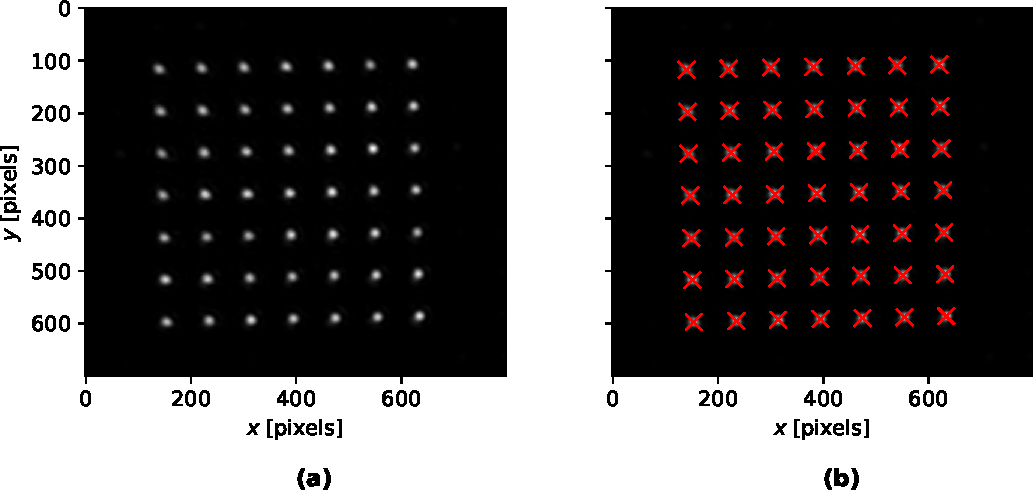
\includegraphics[width=\textwidth]{figures/CamImgLoGSpots.pdf}
    \caption{\textsf{\textbf{a)}} $7\times7$ spot array as obtained from the Flea2 CCD chip.
    \textsf{\textbf{b)}} Spot locations marked with the red crosses, as obtained from the edge-detection algorithm. }
    \label{fig:CameraLoG}
\end{figure}

\begin{equation}\label{eq:2DGaussianNumberK}
    U_m(x,y) = U_{0,m}\exp{\left(\frac{-(x_m-x_{0,m})^2}{2\sigma_{x,m}^2}\right)}
    \exp{\left( \frac{-(y_m-y_{0,m})^2}{2\sigma_{y,}^2} \right)}.
\end{equation}
The fit is similar to the one shown in \cref{fig:3Dshowing}.
Each fit of spot $m$ has 5 fit parameters: the amplitude (optical trap depth) of the Gaussian: $U_{0,m}$, the center of the potential $(x_{0,m}, y_{0,m})$ and lastly the spread of the Gaussian in Cartesian coordinates $\{\sigma_{x,m},\sigma_{y,m}\}$.
Similar to the single tweezer of the previous chapter, the waist is obtained as $w_{0,m} = \sigma_{x,m}+\sigma_{y,m}$, a assumption valid for $\sigma_x\sim\sigma_y$.

In order to routinely perform each fit, a starting guess for the center of each potential is needed, after which a \ac{RoI} can be extracted similar to \cref{fig:3Dwaistfit}.
To reliably detect the expected number of spots, we used the \ac{LoG} edge detection algorithm \cite{Haralick1992}. 
This methods works by computing the second spatial derivative in $x$ and $y$ (Laplacian) of a 2D-array. 
If this second derivative crosses a zero with a slope above a certain user-defined threshold, a feature is marked as an edge (spot).
To prevent noisy pixels from being marked as an edge, the image is first convolved with a Gaussian, smoothing out these pixels. 
We set the Gaussian to have a $\sigma$ roughly the same dimensions as the feature one wishes to detect. 
If the detected number of spots is too little or too high, the detection threshold can be adjusted, which we did not find to be necessary in practice. 
\begin{figure}
    \centering
    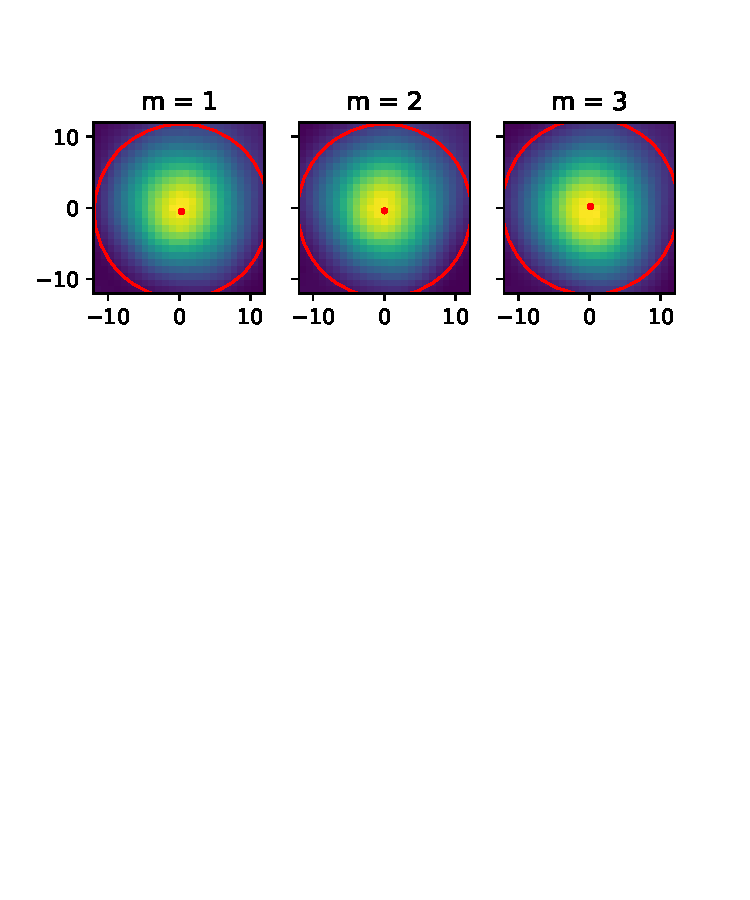
\includegraphics[width=0.62\textwidth]{figures/SpotsCropped_range12.pdf}
    \caption{Region of interest in pixels around the first 3 spots, as extracted by the Laplacian of Gaussian. 
    The centers $(x_{m,0},y_{m,0})$ as found by the 2D least square fit is shown by the red dot. 
    The obtained $1/e^2$ radius $w_{m,0}$ is denoted by the circles is drawn for each peak $m$ as well.}
    \label{fig:SpotsRoI}
\end{figure}

The spots found by the algorithm are marked in \ref{fig:CameraLoG}b by red crosses. 
In \cref{fig:SpotsRoI}, the extracted \ac{RoI} by the \ac{LoG} algorithm is shown for the first 3 peaks. 
Subsequently, the center of the peaks as found by the 2D fit $(x_{0,m},y_{0,m})$ is marked with the red dot, where the $1/e^2$ radii are marked by circles. 
Subsequently, the extracted fit parameters can be used to perform some statistics.
Histograms of the obtained waist as well as trap depths for the same $7\times7$ array are presented in \cref{fig:WaistHistogram,fig:DepthHistogram}.
We fitted the data in the histograms to a normal distribution, yielding a waist of $w_0 = (0.89 \pm 0.03)$ $\mu$m, where the error denotes the standard deviation, and not the uncertainty in the calibration of the magnification. 
This result was approximately identical for all array dimensions tested, including the single tweezer of the previous chapter. 

\begin{figure}
	\begin{subfigure}{.49\linewidth}
		\centering
		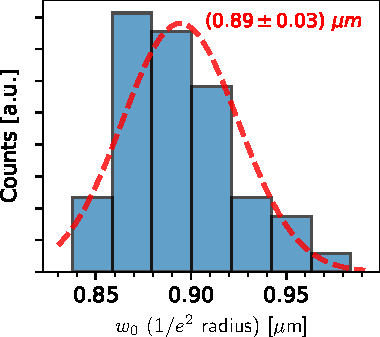
\includegraphics[height=5.9cm]{figures/WaistHistogram.pdf}
		\caption{}
		\label{fig:WaistHistogram}
	\end{subfigure}
	\hfill
	\begin{subfigure}{.49\linewidth}
		\centering
		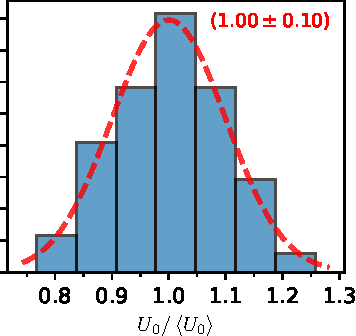
\includegraphics[height=5.9cm]{figures/DepthHistogram.pdf}
		\caption{}
		\label{fig:DepthHistogram}
	\end{subfigure}
	\caption{
	\textsf{\textbf{a)}} Distribution of the $1/e^2$ radius as measured from the spot array in \cref{fig:CameraLoG}a.
   \textsf{\textbf{b)}} Spread in the fitted depth of the potential $U_0$, normalized by the     average trap depth $\left\langle U_0 \right\rangle$.
    Both are fit to a normal distribution.
    }
\end{figure}


As a result of the slightly varying waist, there will also be a non-homogeneity (uniformity) in the intensities (trap depths) of the array.
There are other causes to the spread in uniformity as well.
For example, the diffraction efficiency of the SLM increases as one gets closer to the zeroth order approximately as $\operatorname{sinc}^2\{
\pi (\theta_{\text{m}}/\theta_{\text{m,max}})/2\}$ where $\theta_m$ is the deflection angle from the zeroth order for spot $m$ and $\theta_{m,max}$ is the smallest deflection angle within the array \cite{Ebadi2021}.
Because we used quite a strong linear phase ramp, we are very far from the optical axis and this variation over the will be minimal, however.


The spread in trap depths is shown in \cref{fig:DepthHistogram}.
Because we only care about the spread and not about the magnitude of the intensity (the latter is dependent on camera sensitivity, dichroic filters and laser power used), we normalize by the average trap depth $\left\langle U_0 \right\rangle$, yielding for this array a spread $\sigma_{U_0} / \left\langle U_0 \right\rangle$ of $\sim10$\% after fitting a normal distribution,
It is unlikely that the uniformity is indeed normally distributed, but using the Shapiro-Wilk test we cannot state that the distribution is \textit{not} distributed normally ($p>0.3$ for all array dimensions tested).
In \cref{fig:Uniformity}, we plotted the uniformity as a function of the array size $n\times n$.
Clearly, the non-homogeneity increases with the array dimension $n$: for the $2\times 2$ array it was just $0.9\%$ and for larger arrays we typically see $\sim 10\%$.
This is to be expected, because for larger arrays the hologram on the SLM responsible for generating the spot array will be more complicated. 
Because of the discrete nature of the SLM, it can only approximate rapidly varying phase patterns with high spatial frequencies, leading to discrepancies. 


To our knowledge, there is no literature result of the measurement method used here to compare to, because in a cold atom experiment the array uniformity is usually measured by an imaging system of similar \ac{NA} by

\begin{enumerate}
    \item Placing the camera after the glass cell. 
    In our case that the camera would have to be accompanied be an identical long-working distance microscope objective, to bridge the 30 mm outer thickness of the cell.
    This is the same principle as using a set of two in-vacuum high-NA aspheric lenses as done by \cite{Nogrette2014}.
    
    \item Separating Stark-shifted atomic fluorescence from ultra-cold atoms in tweezers recorded by the same high-NA lens used to produce the tweezer array \cite{Ebadi2021}.
\end{enumerate}
In both cases, the light travels twice through the high-NA lens and vacuum glass, which typically seems to yield a larger spread: \cite{Nogrette2014} found 19\% standard deviation uniformity whereas we found $10\%$.


\begin{figure}
    \centering
    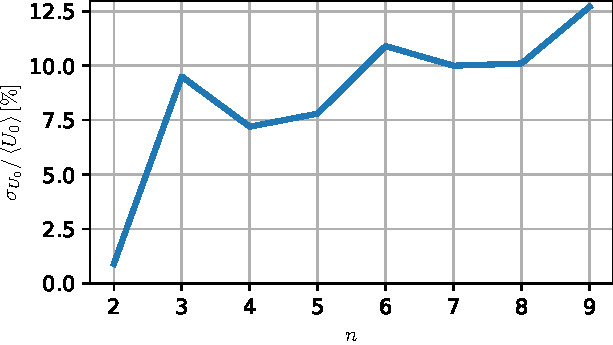
\includegraphics[width=0.6\textwidth]{figures/UniformityAmountsSpots.pdf}
    \caption{Standard deviation of normal distribution fit plotted against the array dimension $\sqrt{n\times n}$ where $n \times n$ is the amount of spots. }
    \label{fig:Uniformity}
\end{figure}
As also shown by \cite{Nogrette2014}, it is also possible to improve this uniformity by iteratively adapting the weight factors in the \ac{GSW} algorithm in a feedback loop to achieve a non-homogeneity of $1.4\%$.
It is worth noting here that this correction can only be as good as the imaging system used to obtain the feedback. 
Thus, in the method 1) one has to be careful not to 'over-correct' for aberrations \cite{Labuhn2016}, as it is impossible to know if the aberrations really occur in the focusing plane of the objective near the atoms, or are rather a result of the imaging system which will also have aberrations. 
Because of this, the latter method 2) of really looking at the Stark shift by the atomic fluorescence might be the more robust method because here the aberration picked up by the imaging system will be approximately the same aberration introduced by producing the tweezer array in the first place (as the same high-NA lens is used.)
Both methods 1) and 2) are possible to implement in our ultra-cold experiment, which we will introduce now.







